\documentclass[a4paper,12pt]{report}
\usepackage{projectreport}
\usepackage{graphicx}
\usepackage{titlesec}
\usepackage{centernot}
\usepackage{titling}
% \usepackage[hidelinks]{hyperref}
% \usepackage[style=ieee]{biblatex}

% \usepackage[style=numeric]{biblatex}

\titleformat{\subsection}
  {\normalfont\fontsize{12}{14}\bfseries}
  {\thesubsection}{1em}{}

% ----------------- Bibliography Setup -----------------
% \addbibresource{references.bib}


% Rename "Bibliography" to "References"
\DefineBibliographyStrings{english}{%
  bibliography = {References},
}

\usepackage[utf8]{inputenc}

\usepackage{newunicodechar}
\newunicodechar{β}{\beta}
\newunicodechar{₁}{$_1$}
\newunicodechar{₂}{$_2$}

\usepackage{pgfplots}
\pgfplotsset{compat=1.18} % Use appropriate version

\usepackage{array}
\setlength{\extrarowheight}{4pt}
\usepackage{tabularx}

\usepackage{blindtext}
\usepackage[utf8]{inputenc}
\usepackage{geometry}
\usepackage{ragged2e}
\usepackage{fancyhdr}
\usepackage{array}
\usepackage{titlesec}
\usepackage{tikz}
\usetikzlibrary{shapes.geometric, arrows}

\tikzstyle{startstop} = [rectangle, rounded corners, minimum width=2.5cm, minimum height=1cm, text centered, draw=black, fill=red!30, font=\small]
\tikzstyle{process} = [rectangle, minimum width=3cm, minimum height=1cm, text centered, draw=black, fill=blue!30, font=\small]
\tikzstyle{decision} = [diamond, minimum width=2.5cm, minimum height=1cm, text centered, draw=black, fill=green!30, font=\small]
\tikzstyle{arrow} = [thick,->,>=stealth]

\pagestyle{fancy}

\newcounter{boldsection}
\newcommand{\centerheading}[1]{%
  \refstepcounter{boldsection}%
  \par\noindent\textbf{\LARGE \theboldsection.\ #1}\par\vspace{0.5em}
}

\geometry{a4paper, top=1in, bottom=20mm}
\usepackage{subcaption} % Needed for subfigure environment

% Title formatting
\titleformat{\chapter}[display]
  {\normalfont\fontsize{22}{18}\bfseries\centering}
  {\chaptername\ \thechapter}
  {20pt}
  {\Huge}


\titleformat{\section}
  {\normalfont\fontsize{14}{16}\bfseries}
  {\thesection}{1em}{}


\titleformat{\subsection}
  {\normalfont\fontsize{12}{14}\bfseries}
  {\thesubsection}{1em}{}


% Left-align the References heading and add it to TOC
\defbibheading{bibliography}[\refname]{%
  \section*{#1}
  \addcontentsline{toc}{section}{#1}
}


\renewcommand{\contentsname}{Table of Contents}

\newcommand{\notocsection}[1]{%
  \refstepcounter{section}%
  \section*{\thesection\quad#1}%
}

\usepackage{listings}
\usepackage{xcolor}

\lstset{
    basicstyle=\ttfamily\small,
    keywordstyle=\color{blue}\bfseries,
    commentstyle=\color{gray}\itshape,
    stringstyle=\color{red},
    showstringspaces=false,
    numbers=left,
    numberstyle=\tiny\color{gray},
    breaklines=true,
    frame=single,
    tabsize=2,
    captionpos=b
}


\begin{document}

% ----------------- Cover Page -----------------
\begin{titlepage}
    \centering
    \textbf{\Large Capstone Project-1(CSEE-612P) Report on}\\[0.3cm]
    \rule{\linewidth}{0.3mm} \\[0.2cm]
    {\LARGE \textbf{ Enhanced Image Resolution Using GANs}} \\[0.1cm]
    \rule{\linewidth}{0.3mm} \\[0.5cm]
    
    \textbf{Submitted in partial fulfilment of the requirement for the award of the degree of}\\[0.1cm]
    \textbf{BACHELOR OF TECHNOLOGY}\\[0.1cm]
    \textbf{IN}\\[0.1cm]
    \textbf{COMPUTER SCIENCE \& ENGINEERING\\
    (AI\&ML)}\\[0.5cm]
    
    \textbf{Submitted by:}\\[0.3cm]
    
\begin{tabular}{@{}l@{\hspace{2cm}}l@{}}
    \textbf{Student Name} & \textbf{University Roll No.} \\
    Ayush Raina & 22010103014 \\
    Bharat Bhushan & 22010103016 \\
    Jatin Sharma & 22010103022 \\
    Kanishk Thakur & 22010103025 \\
    Karan & 22010103026 \\
    Nancy & 22010103033 \\
    Nikunj Lohia & 22010103035 \\
    Rishita & 22010103044 \\
    Riya Thakur & 22010103047 \\
    Tanishq Sohal & 22010103071 \\
\end{tabular}\\[1cm]

    \textit{Under the Mentorship of}\\[0.2cm]
    \textbf{Er. Aditi}\\
    \textbf{Assistant Professor}\\[0.4cm]
    
    
\includegraphics[width=4cm]{image/jngec.jpg} \\
    \vspace{0,7cm}

    \textbf{Department of Computer Science and Engineering}\\[0.1cm]
    \textbf{Jawaharlal Nehru Govt. Engineering College }\\[0cm]
    \textbf{Sundernagar, Mandi, HP}\\[0.15cm]
    \textbf{(2024-25)}
\end{titlepage}

% ----------------- Roman Page Numbering Starts Here -----------------
\pagenumbering{roman}
\setcounter{page}{0}

% ----------------- Candidate’s Declaration Page -----------------
\thispagestyle{empty}
\begin{center}
    {\Large \textbf{CANDIDATE’S DECLARATION}}\\[1.5cm]
\end{center}

\noindent
We hereby certify that the work which is being presented in the project report entitled \textbf{“Enhanced Image Resolution Using GANs”} in partial fulfillment of the requirements for the award of the Degree of Bachelor of Technology in Computer Science and Engineering(AI\&ML) of Jawaharlal Nehru Government Engineering College, Sundernagar, has been carried out by us under the mentorship of \textbf{Er. Aditi, Assistant Professor}, Department of Computer Science and Engineering(AI\&ML), Jawaharlal Nehru Government Engineering College, Sundernagar.

% \vspace{1.2cm}

% \noindent\textbf{Submitted by:}

\vspace{0.5cm}
\begin{tabular}{ll}
\textbf{Student Name} & \textbf{University Roll No.}\\
Ayush Raina & 22010103014 \\
Bharat Bhushan & 22010103016 \\
Jatin Sharma & 22010103022 \\
Kanishk Thakur & 22010103025 \\
Karan & 22010103026 \\
Nancy & 22010103033 \\
Nikunj Lohia & 22010103035 \\
Rishita & 22010103044 \\
Riya Thakur & 22010103047 \\
Tanishq Sohal & 22010103071 \\
\end{tabular}

\vspace{2cm}
% \noindent
% Date: \hfill Signatures of Candidates

% ----------------- Table of Contents -----------------
% ----------------- Table of Contents -----------------
\newpage
\thispagestyle{empty}
\tableofcontents

\clearpage
\pagenumbering{roman}  % Set page numbering to Arabic
\setcounter{page}{1}    % Reset page number to 1

\addcontentsline{toc}{section}{List of Figures}
\listoffigures

\clearpage
\addcontentsline{toc}{section}{List of Tables}
\listoftables

\clearpage

% \lstlistoflistings	
% \addcontentsline{toc}{section}{Introduction}
\newpage
\fancypagestyle{noheader}{
  \fancyhf{}
  \fancyfoot[C]{\thepage}
}
\pagestyle{noheader}

\begin{center}
    \textbf{\Large List of Abbreviations}
\end{center}

\vspace{1em}
\addcontentsline{toc}{section}{List of Abbreviations}

\begin{center}
\begin{tabular}{|p{3cm}|p{11cm}|}
\hline
\textbf{Abbreviation} & \textbf{Full Form} \\
\hline
GANs & Generative Adversarial Networks \\
CNNs & Convolutional Neural Networks \\
AI\&ML & Artificial Intelligence \& Machine Learning \\
SR & Super-Resolution \\
SRCNN & Super-Resolution Convolutional Neural Network \\
VDSR & Very Deep Super-Resolution \\
DRCN & Deeply-Recursive Convolutional Network \\
SRGAN & Super-Resolution Generative Adversarial Network \\
VGG & Visual Geometry Group \\
EDSR & Enhanced Deep Super-Resolution \\
LapSRN & Laplacian Pyramid Super-Resolution Network \\
ESRGAN & Enhanced Super-Resolution Generative Adversarial Network \\
Real-ESRGAN & Real-World Enhanced Super-Resolution Generative Adversarial Network \\
SwinIR & Swin Transformer for Image Restoration \\
RRDB & Residual-in-Residual Dense Block \\
RCAN & Residual Channel Attention Network \\
TPE-GAN & Thumbnail Preserving Encryption GAN \\
Atten-GAN & Attention-Based Generative Adversarial Network for Trajectory Prediction \\
SSIM & Structural Similarity Index Measure \\
PSNR & Peak Signal-to-Noise Ratio \\
DIV2K & Dataset for Image and Video Super-Resolution \\
LR & Low Resolution \\
HR & High Resolution \\
L1 Loss & Mean Absolute Error Loss \\
\hline
\end{tabular}
\end{center}


\pagestyle{fancy}


% ----------------- Switch to Arabic Page Numbering -----------------
\clearpage
\pagenumbering{arabic}
\setcounter{page}{1}

% ----------------- Chapters -----------------

\chapter{Introduction} % enter the name of the chapter here
\label{cha:chapter label} % enter the chapter label here (for cross referencing)


% \section*{Introduction}
Generative Adversarial Networks (GANs) are a powerful deep learning framework introduced by Ian Goodfellow and his colleagues in 2014. They are widely used in generative modeling tasks such as image synthesis, image super-resolution, style transfer, and data augmentation. GANs are unique in their architecture because they consist of two competing neural networks—the Generator and the Discriminator—which are trained simultaneously in an adversarial manner.

\begin{figure}[h!]
    \centering
    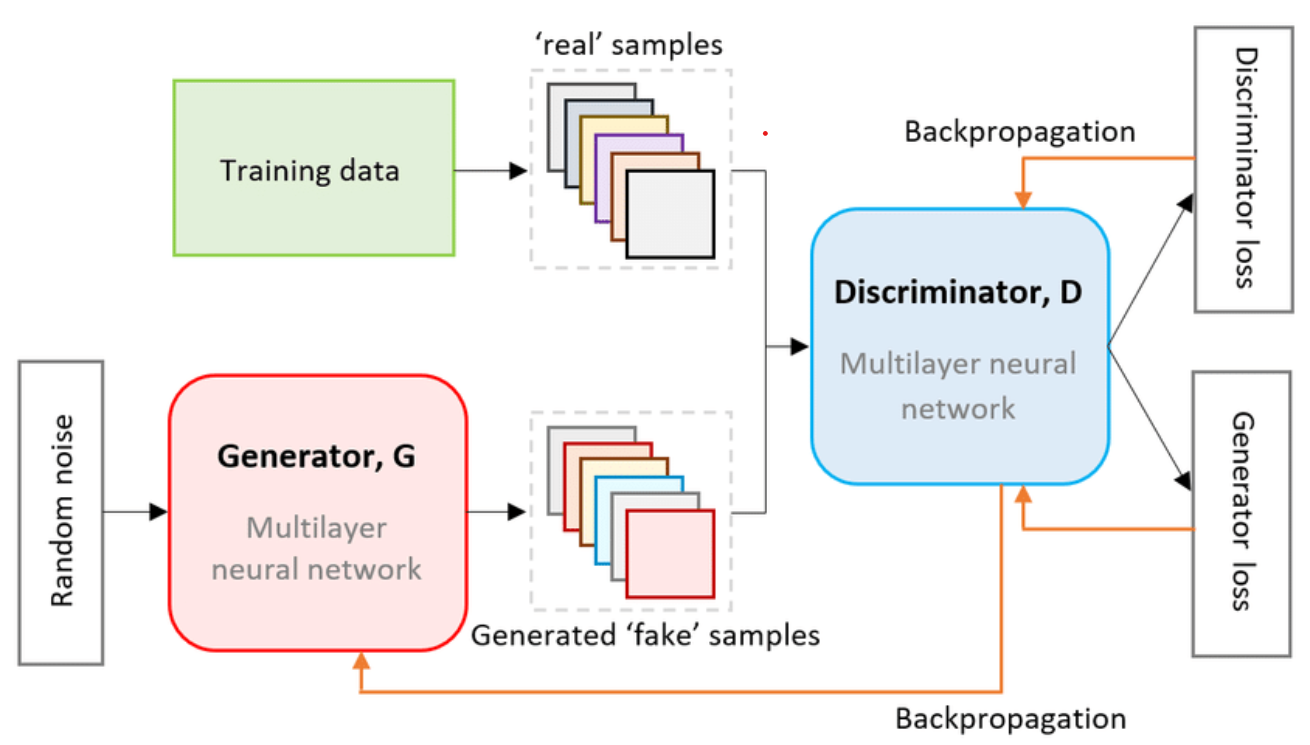
\includegraphics[width=0.7\textwidth]{image/arch.png} % <-- Update with your actual file path
    \caption{GAN Architecture}
    \label{fig:workflow}
\end{figure}
% \subsection*{Components of a GAN}

% A typical Generative Adversarial Network (GAN) consists of two main components:

\begin{itemize}
    \item \textbf{Generator (G):} The generator takes a random noise vector (or a low-resolution image in the case of super-resolution) as input and transforms it into a high-resolution or realistic-looking image. It uses transposed convolution layers or upsampling layers to increase the spatial dimensions of the image and is trained to produce outputs that look as real as possible to the discriminator.
    
    \item \textbf{Discriminator (D):} The discriminator is a binary classifier that takes an image as input and outputs the probability of whether the image is real (from the dataset) or fake (generated by the generator). It uses convolutional layers to extract features and is trained to correctly classify the images.
\end{itemize}

Both the generator and discriminator are trained simultaneously using a minimax loss function:

\begin{equation}
    \min_G \max_D \; \mathbb{E}_{x \sim p_{\text{data}}(x)} [\log D(x)] + \mathbb{E}_{z \sim p_z(z)} [\log(1 - D(G(z)))]
\end{equation}

Here:
\begin{itemize}
    \item $x$ is a real data sample from the true data distribution $p_{\text{data}}$.
    \item $z$ is a noise vector sampled from a prior distribution $p_z$ (e.g., uniform or Gaussian).
    \item $G(z)$ is the image generated by the generator from noise $z$.
    \item $D(x)$ is the probability output by the discriminator that $x$ is a real image.
\end{itemize}
\vspace{0.07cm}
\textbf{Convolutional Neural Networks (CNNs):}\\
Convolutional Neural Networks (CNNs) are a class of deep learning models particularly well-suited for image processing tasks. They use convolutional layers to automatically learn spatial hierarchies of features from input images. CNNs are effective at tasks like image classification and object detection, but in image super-resolution, they often produce blurry results due to their reliance on pixel-wise losses. Unlike GANs, CNNs lack the ability to generate high-frequency details and perceptual realism.


% \section{Objective:}
% \begin{itemize}
%     \item To study and implement GANs for enhancing image resolution.
  

% \item To develop a technique that transforms low-resolution images into high
% resolution outputs.

% \item To evaluate the performance of the model on datasets relevant to medical
%  imaging, streaming, and security.
% \end{itemize} 

\section{Problem statement}
The aim of this project is to address the challenge of generating high-resolution images from low-resolution inputs using a deep learning approach. Specifically, the project seeks to implement and evaluate the Enhanced Super-Resolution Generative Adversarial Network (ESRGAN) to reconstruct visually pleasing and high-quality images, thereby overcoming the limitations of conventional interpolation methods.

% \section{What is the problem}
% In many practical applications like satellite imaging, medical diagnostics, video surveillance, and old photo restoration, the available images are often of low quality or resolution. Traditional image upscaling techniques such as bicubic interpolation often result in blurry or pixelated images with loss of texture and fine details. The problem is to create a system that can enhance image resolution while preserving fine textures, edges, and realistic details, thus improving the overall visual quality.

\section{Why is this a project related to this class}
This project relates directly to the subjects of Machine Learning, Deep Learning, and Computer Vision, which are essential components of the curriculum in Computer Science and Engineering(AI\&ML). It involves the use of Neural Networks, Generative Adversarial Networks (GANs), image processing, and data-driven model training, which align with the theoretical and practical knowledge imparted in these courses. The project also builds hands-on experience with frameworks like PyTorch or TensorFlow, strengthening both academic and industry-ready skills.

\section{Area or Scope of Investigation}
\begin{itemize}
    % \item Domain: Deep Learning, Computer Vision, Image Processing
    
    % \item Tools \& Technologies: Python, PyTorch, Matplotlib, PIL, ESRGAN architecture
    
    % \item Dataset Used: DIV2K (high-resolution image dataset used for super-resolution tasks)
    
    % \item Scope:
    % \begin{itemize}
        \item Training ESRGAN on real-world image datasets.
        \item Understanding the internal architecture of GANs and their applications.
        \item Visualizing and analyzing the results using graphs and image comparisons.
        \item Enhancing the project to real-time applications such as video upscaling or photo enhancement tools in the future.
    % \end{itemize}
\end{itemize}

\chapter{Literature Survey}

Several researchers have contributed significant work in the field of image super-resolution. Various deep learning-based models such as CNNs and GANs have been proposed to enhance image quality by learning high-frequency features. The following studies represent some of the prominent developments in this area.
\vspace{0.5cm}

\textbf{CNN-based Super-Resolution:}

Dong et al. (2014) \cite{a2} introduced SRCNN, the first deep learning-based SR model using convolutional neural networks (CNNs). SRCNN demonstrated significant performance improvements over previous methods in terms of PSNR and SSIM. It was later followed by deeper architectures such as VDSR (Kim et al., 2016) and DRCN, which leveraged residual learning to further enhance results. \cite{a3}

\vspace{0.3cm}

\textbf{GAN-based Super-Resolution:}


\textbf{Lai et al. (2017)} \cite{a10}Proposed a Laplacian pyramid network structure for progressive image reconstruction with improved accuracy and speed.(LapSRN)

\textbf{Ledig et al. (2017)} \cite{a4} proposed the SRGAN model, which marked a major milestone in perceptual super-resolution. SRGAN combined an adversarial loss with perceptual loss derived from VGG networks, resulting in photo-realistic high-resolution images.

\textbf{Lim et al. (2017)} \cite{a9}Removed unnecessary modules from traditional residual networks, allowing for deeper and more efficient SR models.(EDSR) 

\textbf{Wang et al. (2018)} \cite{a5}Enhanced the SRGAN framework by introducing Residual-in-Residual Dense Blocks (RRDB) and a relativistic discriminator.(ESRGAN) 

\textbf{Zhang et al. (2018)} \cite{a8}Introduced a channel attention mechanism to adaptively rescale channel-wise features for improved high-frequency detail restoration.(RCAN) 

\textbf{Liang et al. (2021)} \cite{a7}Utilized Swin Transformers for SR, achieving state-of-the-art results on multiple benchmarks.(SwinIR)


\textbf{Wang et al. (2021)} \cite{a6}Aimed at real-world image SR by handling unknown degradations using a generalized degradation model.(Real-ESRGAN)

\textbf{Chai et al. (2022)} \cite{a11} Proposed TPE-GAN, a GAN-based method for image encryption that preserves thumbnails while ensuring security through key-based access. (TPE-GAN)

\textbf{Fang et al. (2022)} \cite{a12} Introduced Atten-GAN for pedestrian trajectory prediction by incorporating attention mechanisms into GANs to improve contextual understanding. (Atten-GAN)
\chapter{Methodology}

\notocsection{Dataset Acquistion}
To train a super-resolution model, it is crucial to collect relevant datasets comprising low-resolution (LR) images. These images can be obtained by downsampling high-resolution (HR) images using bicubic interpolation
\begin{itemize}
    \item The DIV2K dataset is used, which contains 800 high-resolution training images and corresponding low-resolution images created using bicubic downsampling.
    % \item Images are preprocessed to ensure compatibility with the ESRGAN input format (e.g., resizing, normalization).
\end{itemize}


The datasets should be split into training, validation, and testing sets to ensure effective evaluation and avoid overfitting.
\begin{figure}[h!]
    \centering
    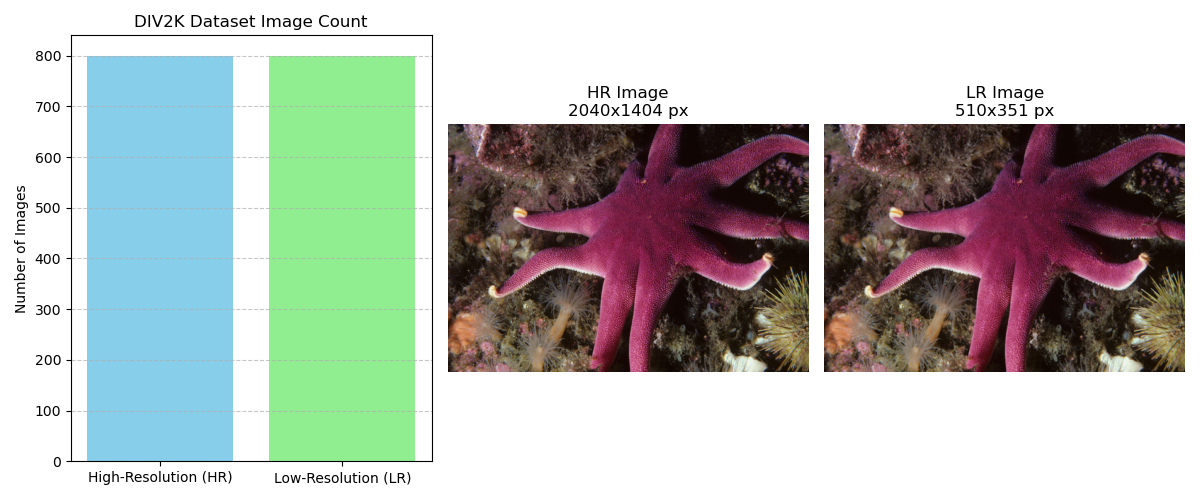
\includegraphics[width=1\textwidth]{image/Figure_1.png} % <-- Update with your actual file path
    \caption{DIV2K Dataset}
    \label{fig:workflow}
\end{figure}

\notocsection{Data Preprocessing}
Before training the model, all images undergo preprocessing to ensure consistency:
\begin{itemize}
    \item \textbf{Resizing}: Images are downsampled to create LR-HR image pairs.
    \item \textbf{Normalization}: Pixel values are scaled to the range $[0, 1]$  depending on the activation function used in the neural network.
    \item \textbf{Data Augmentation}: Techniques such as rotation, flipping, and cropping help in increasing the diversity of the training data.
\end{itemize}
\vspace{0.5cm}

\notocsection{Execution and Designing of GAN}
A Generative Adversarial Network (GAN) is composed of two primary components:

\textbf{1. Generator: }We built a deep generator using Residual-in-Residual Dense Blocks (RRDB), capable of learning fine image textures. It accepts low-resolution (LR) images and upscales them to high-resolution (HR) outputs using learned features and two upsampling layers.
    
\textbf{2. Discriminator:} A deep CNN-based network that classifies between real HR images and those generated by the generator. It is trained adversarially to improve perceptual quality.

\vspace{0.7cm}
    
% \textbf{Loss Functions:}
    
    % \begin{itemize}
    %     \item Perceptual Loss: Implemented using a pre-trained VGG19 network to compute feature-based loss.
        
    %     \item Adversarial Loss: Helps the generator produce more realistic outputs.
        
    %     \item Pixel Loss (L1): Encourages similarity between generated and real images at pixel level.
        
    % \end{itemize}
% We trained the model using the Wasserstein GAN with Gradient Penalty approach to ensure stable training and better visual results. The ESRGAN model was trained for 100 epochs and compared with a CNN baseline to validate its effectiveness.The generator is trained to fool the discriminator while the discriminator learns to better distinguish between real and generated images.

\notocsection{Training and Fine-Tuning}
In this project, we trained the ESRGAN model on the DIV2K dataset in two stages:

\textbf{Initial Training:}

Stabilize the generator before introducing adversarial loss.

Trained the generator alone for 100 epochs using only the L1 (pixel) loss.

\textbf{Settings:}

\begin{itemize}
    \item Optimizer: Adam (learning rate 1e-4, $\beta$₁=0.9, $\beta$₂=0.999)
    \item Batch size: 8
    \item LR scheduling: Reduce by factor of 10 at epoch 50
\end{itemize}

\textbf{Adversarial Fine-Tuning}

Improve perceptual fidelity by introducing the discriminator and perceptual loss.

Jointly trained generator and discriminator for 200 additional epochs.

\textbf{Settings:}

\begin{itemize}
    \item Discriminator updates per generator update: 1
    \item Loss weights: 1.0·L1, 2e-6·Perceptual, 1e-3·Adversarial
    \item Learning rate kept at 1e-4, halved at epoch 100
\end{itemize}


% The training process involves multiple loss functions:
% \begin{itemize}
%     \item \textbf{Adversarial Loss} ($\mathcal{L}_{adv}$): Encourages the generator to produce perceptually realistic images.
%     \item \textbf{Perceptual Loss} ($\mathcal{L}_{perc}$): Uses feature maps from a pretrained network (e.g., VGG) to ensure perceptual similarity.
%     \item \textbf{Content Loss} ($\mathcal{L}_{content}$): Based on pixel-wise differences such as L1 or L2 loss between generated and real images.
% \end{itemize}
% The total loss function is a weighted sum of these components:
% \[
% \mathcal{L}_{total} = \lambda_{adv} \mathcal{L}_{adv} + \lambda_{perc} \mathcal{L}_{perc} + \lambda_{content} \mathcal{L}_{content}
% \]

\notocsection{Evaluation}
The performance of the super-resolution GAN is measured using standard image quality metrics:
\begin{itemize}
    \item \textbf{PSNR (Peak Signal-to-Noise Ratio)}: Measures the ratio between the maximum possible power of a signal and the power of corrupting noise.
    \item \textbf{SSIM (Structural Similarity Index)}: Evaluates the similarity between the generated and ground truth images based on luminance, contrast, and structure.
    o further validate image fidelity, we converted grayscale versions of the SR and HR images into binary representations and computed the following:

\item \textbf{Precision:}
Precision evaluates the proportion of predicted positive pixels that were actually correct. High precision indicates fewer false positives in the generated images.

\item \textbf{Recall:}
Recall measures the ability of the model to capture all the relevant high-frequency details. Our model achieved high recall values, showing it effectively preserved essential visual information.

\item \textbf{F1 Score:}
F1 Score is the harmonic mean of precision and recall, providing a balance between the two. A strong F1 score in our results reflects the overall accuracy of the GAN-generated images in replicating the ground truth.
\end{itemize}
% Higher PSNR and SSIM values typically indicate better quality reconstruction.
\vspace{0.5cm}

% \section{Application and Validation}
% Once trained and evaluated, the model can be deployed in practical applications:
% \begin{itemize}
%     \item \textbf{Medical Imaging}: Enhancing MRI or CT scans for better diagnosis.
%     \item \textbf{Surveillance Systems}: Improving the clarity of footage captured from low-resolution security cameras.
%     \item \textbf{Streaming Platforms}: Enhancing video quality for improved viewing experience in low bandwidth conditions.
% \end{itemize}
% \begin{figure}[h!]
%     \centering
%     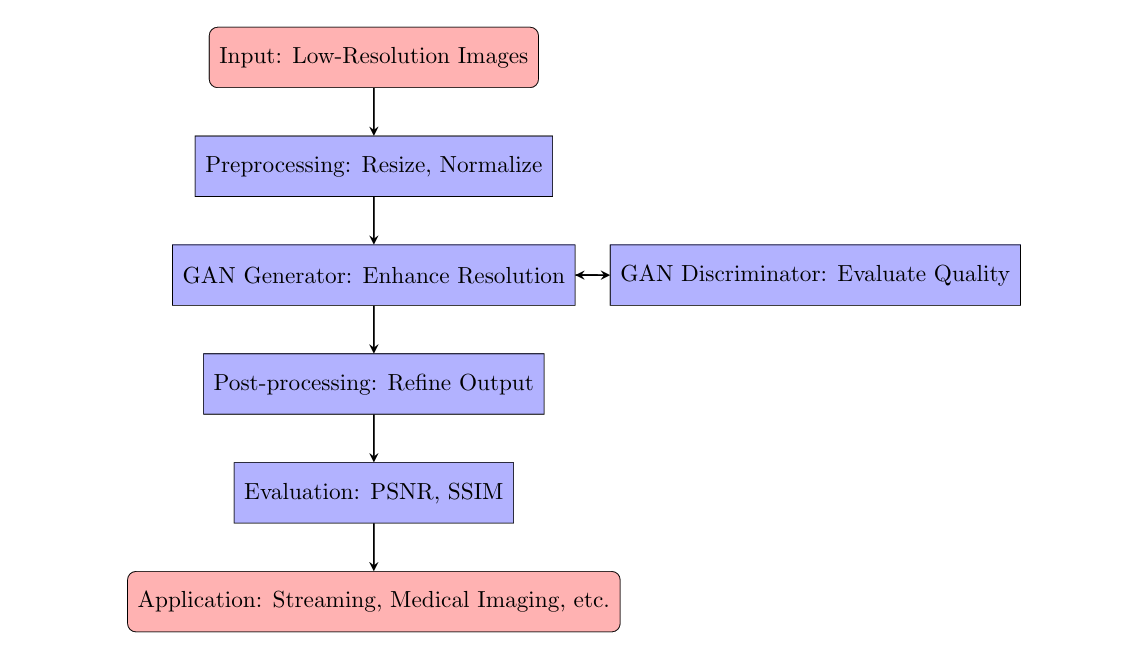
\includegraphics[width=1\textwidth]{workflow.png} % <-- Update with your actual file path
%     \caption{Workflow diagram of the proposed super-resolution methodology.}
%     \label{fig:workflow}
% \end{figure}
% The effectiveness of the model can be validated by comparing the performance of real-world tasks (e.g., object detection accuracy) before and after applying super-resolution.


% \begin{center}

% \begin{tikzpicture}[node distance=1.8cm]

% % Nodes
% \node (start) [startstop] {Input: Low-Resolution Images};
% \node (preprocess) [process, below of=start] {Preprocessing: Resize, Normalize};
% \node (generator) [process, below of=preprocess] {GAN Generator: Enhance Resolution};
% \node (discriminator) [process, right of=generator, xshift=5.5cm] {GAN Discriminator: Evaluate Quality};
% \node (postprocess) [process, below of=generator] {Post-processing: Refine Output};
% \node (finetuning) [process, below of=postprocess] {Post-processing: Refine Output};
% \node (evaluate) [process, below of=postprocess] {Evaluation: PSNR, SSIM};
% % \node (application) [startstop, below of=evaluate] {Application: Streaming, Medical Imaging, etc.};

% % Arrows
% \draw [arrow] (start) -- (preprocess);
% \draw [arrow] (preprocess) -- (generator);
% \draw [arrow] (generator) -- (postprocess);
% \draw [arrow] (postprocess) -- (finetuning);
% \draw [arrow] (finetuning) -- (evaluate);
% % \draw [arrow] (evaluate) -- (application);
% \draw [arrow] (generator.east) -- (discriminator.west);
% \draw [arrow] (discriminator.west) ++(-0.2,0) |- (generator.east);

% \end{tikzpicture}
% \end{center}
\notocsection{GAN Implementation}
In this project, we implemented an Enhanced Super-Resolution Generative Adversarial Network (ESRGAN) to convert low-resolution images into high-resolution outputs. The implementation involved the following major steps:

\begin{itemize}
    \item \textbf{Generator Network:} Designed using Residual-in-Residual Dense Blocks (RRDB), the generator takes low-resolution images as input and learns to produce perceptually accurate high-resolution images. It includes deep convolutional layers, skip connections, and upsampling blocks to preserve fine details.
    
    \item \textbf{Discriminator Network:} A convolutional neural network (CNN) that distinguishes between real high-resolution images and generated images. It guides the generator to produce more realistic outputs through adversarial training.
    
    \item \textbf{Loss Functions:} The model was trained using a combination of adversarial loss, L1 loss, and VGG perceptual loss. This ensured that the generated images were not only visually realistic but also structurally similar to the original high-resolution images.

    \textbf{1. Adversarial Loss (0.866):} Indicates how effectively the generator is able to fool the discriminator. A positive value shows that the generator is learning meaningful features and successfully confusing the discriminator.

\textbf{2. Critic Loss / Wasserstein Distance (25.4):} Represents the ability of the discriminator to distinguish between real and generated images. Higher values suggest better discrimination capability, which guides the generator to improve further.

\textbf{3. Gradient Penalty (0.894):} Used to enforce the Lipschitz constraint in WGAN-GP. A stable and low gradient penalty ensures smoother and more stable training dynamics.

\textbf{4. L1 Loss (0.00235): }Measures the average pixel-wise error between generated and real high-resolution images. A low L1 loss indicates high fidelity in pixel-level reconstruction.

\textbf{5. VGG Perceptual Loss (2.55):} Quantifies the perceptual similarity using high-level features extracted from a pre-trained VGG19 network. Lower values imply that the generated images closely resemble the ground truth in terms of content and texture.
\vspace{0.5cm}
\end{itemize}


% \begin{center}
% \begin{tikzpicture}[node distance=1.9cm]

% % Node styles (if not already defined in your preamble)
% \tikzstyle{startstop} = [rectangle, rounded corners, minimum width=3cm, minimum height=1cm,text centered, draw=black, fill=blue!20]
% \tikzstyle{process} = [rectangle, minimum width=3cm, minimum height=1cm, text centered, draw=black, fill=orange!30]
% \tikzstyle{arrow} = [thick,->,>=stealth]

% % Nodes
% \node (start) [startstop] {Input: Low-Resolution Images};
% \node (preprocess) [process, below of=start] {Preprocessing: Resize, Normalize};
% \node (generator) [process, below of=preprocess] {GAN Generator: Enhance Resolution};
% \node (discriminator) [process, right of=generator, xshift=6.1cm] {GAN Discriminator: Evaluate Quality};
% \node (postprocess) [process, below of=generator] {Training and Fine-Tuning};
% \node (evaluate) [process, below of=postprocess] {Evaluation: PSNR, SSIM};
% \node (implementation) [process, below of=evaluate] {GAN Implementation};

% % Arrows
% \draw [arrow] (start) -- (preprocess);
% \draw [arrow] (preprocess) -- (generator);
% \draw [arrow] (generator) -- (postprocess);
% \draw [arrow] (postprocess) -- (evaluate);
% \draw [arrow] (evaluate) -- (implementation);
% \draw [arrow] (generator.east) -- (discriminator.west);
% \draw [arrow] (discriminator.south) |- ++(0,-0.6) -| (generator.south);

% \end{tikzpicture}
% \end{center}
% \hspace{3cm} \large{:- Workflow of SRGAN}
% \vspace{0.6cm}

\begin{figure}[h!]
    \centering
    \includegraphics[width=1\textwidth]{Fig3.2.png} % <-- Update with your actual file path
    \caption{Workflow of SRGAN}
    \label{fig:workflow}
\end{figure}

\noindent The methodology for the proposed GAN-based super-resolution system is illustrated in the workflow diagram above. It outlines the key steps, from dataset acquisition to evaluation and GAN Implementation.


The process begins with the acquisitions and preprocessing of low-resolution images. These images are then passed through a GAN-based model, where the generator attempts to reconstruct high-resolution images while the discriminator evaluates their realism. The model is trained using a combination of adversarial, perceptual, and pixel-wise losses. Finally, the results are evaluated using metrics such as PSNR and SSIM to validate performance.

\large\textbf{Implementation}

\begin{lstlisting}[language=Python, caption={ESRGAN Inference Code}]
import os
for dirname, _, filenames in os.walk('/kaggle/input'):
    print(dirname)

from PIL import Image

import numpy as np
from tqdm import tqdm

import cv2
import matplotlib.pyplot as plt

import torch
import torch.nn as nn
from torch.utils.data import Dataset, DataLoader
import torchvision
import torchvision.transforms as transforms
from torchvision.models import vgg19

import albumentations as A
from albumentations.pytorch import ToTensorV2

class SRDataset(Dataset):
    def __init__(self, root_dir, lowres_transform, highres_transform, both_transform):
        super(SRDataset, self).__init__()

        self.root_dir = root_dir

        self.lowres_transform = lowres_transform
        self.highres_transform = highres_transform
        self.both_transform = both_transform

        self.list_of_files = os.listdir(os.path.join(root_dir))

    def __len__(self):
        return len(self.list_of_files)

    def __getitem__(self, index):
        image = cv2.imread(os.path.join(self.root_dir, self.list_of_files[index]))
        image = cv2.cvtColor(image, cv2.COLOR_BGR2RGB)

        image = self.both_transform(image=image)['image']
        low_res_image = self.lowres_transform(image=image)['image']
        high_res_image = self.highres_transform(image=image)['image']

        return low_res_image, high_res_image

class ConvBlock(nn.Module):
    def __init__(self, in_channels, out_channels, use_act, kernel_size=3, stride=1, padding=1):
        super().__init__()
        self.cnn = nn.Conv2d(
            in_channels,
            out_channels,
            kernel_size=kernel_size,
            stride=stride,
            padding=padding
        )
        self.act = nn.LeakyReLU(0.2, inplace=True) if use_act else nn.Identity()

    def forward(self, x):
        return self.act(self.cnn(x))

class UpsampleBlock(nn.Module):
    def __init__(self, in_channels, scale_factor=2):
        super().__init__()
        self.upsample = nn.Upsample(scale_factor=scale_factor, mode="nearest")
        self.conv = nn.Conv2d(in_channels, in_channels, 3, 1, 1, bias=True)
        self.act = nn.LeakyReLU(0.2, inplace=True)

    def forward(self, x):
        return self.act(self.conv(self.upsample(x)))



class DenseResidualBlock(nn.Module):
    def __init__(self, in_channels, channels=32, residual_beta=0.2):
        super().__init__()
        self.residual_beta = residual_beta
        self.blocks = nn.ModuleList()

        for i in range(5):
            self.blocks.append(
                ConvBlock(
                    in_channels + channels*i,
                    channels if i <= 3 else in_channels,
                    kernel_size=3,
                    stride=1,
                    padding=1,
                    use_act=True if i <=3 else False,
                )
            )

    def forward(self, x):
        new_inputs = x
        for block in self.blocks:
            out = block(new_inputs)
            new_inputs = torch.cat([new_inputs, out], dim=1)

        return self.residual_beta * out + x

class RRDB(nn.Module):
    def __init__(self, in_channels, residual_beta=0.2):
        super().__init__()
        self.residual_beta = residual_beta
        self.rrdb = nn.Sequential(*[DenseResidualBlock(in_channels) for _ in range(3)])

    def forward(self, x):
        return self.rrdb(x) * self.residual_beta + x

class Generator(nn.Module):
    def __init__(self, in_channels=3, num_channels=64, num_blocks=23):
        super().__init__()
        self.initial = nn.Conv2d(
            in_channels=in_channels,
            out_channels=num_channels,
            kernel_size=3,
            stride=1,
            padding=1,
            bias=True
        )
        self.residuals = nn.Sequential(*[RRDB(num_channels) for _ in range(num_blocks)])
        self.conv = nn.Conv2d(num_channels, num_channels, kernel_size=3, stride=1, padding=1)
        self.upsamples = nn.Sequential(
            UpsampleBlock(num_channels),
            UpsampleBlock(num_channels)
        )
        self.final = nn.Sequential(
            nn.Conv2d(num_channels, num_channels, kernel_size=3, stride=1, padding=1, bias=True),
            nn.LeakyReLU(0.2, inplace=True),
            nn.Conv2d(num_channels, in_channels, kernel_size=1, stride=1, padding=0, bias=True)
        )

    def forward(self, x):
        initial = self.initial(x)
        out = self.residuals(initial)
        out = self.conv(out) + initial
        out = self.upsamples(out)
        out = self.final(out)
        return out

class Discriminator(nn.Module):
    def __init__(self, in_channels=3, features=(64, 64, 128, 128, 256, 256, 512, 512)):
        super().__init__()

        self.in_channels = in_channels
        self.features = list(features)

        blocks = []

        for idx, feature in enumerate(self.features):
            blocks.append(
                ConvBlock(
                    in_channels=in_channels,
                    out_channels=feature,
                    kernel_size=3,
                    stride=1 + idx % 2,
                    padding=1,
                    use_act=True
                )
            )
            in_channels=feature

        self.blocks = nn.Sequential(*blocks)

        self.classifier = nn.Sequential(
            nn.AdaptiveAvgPool2d((6, 6)),
            nn.Flatten(),
            nn.Linear(in_features=512*6*6, out_features=1024),
            nn.LeakyReLU(0.2, inplace=True),
            nn.Linear(in_features=1024, out_features=1)
        )
        self.sigmoid = nn.Sigmoid()

    def forward(self, x):
        features = self.blocks(x)
        out = self.classifier(features)
        # out = self.sigmoid(out)
        return out

def init_weights(model, scale=0.1):
    for m in model.modules():
        if isinstance(m, nn.Conv2d):
            nn.init.kaiming_normal_(m.weight.data)
            m.weight.data *= scale
        elif isinstance(m, nn.Linear):
            nn.init.kaiming_normal_(m.weight.data)
            m.weight.data *= scale

def test_size():
    gen = Generator()
    disc = Discriminator()
    low_res = 24
    x = torch.randn((5, 3, low_res, low_res))
    gen_out = gen(x)
    disc_out = disc(x)

    print(gen_out.shape)
    print(disc_out.shape)

test_size()
\end{lstlisting}

\chapter{Result and Discussion}
\notocsection{Evaluation Metrics Overview}
To assess the performance of the Super-Resolution Generative Adversarial Network (SRGAN) model, both quantitative and qualitative metrics were utilized:

\textbf{Quantitative Metrics}
\begin{itemize}
    \item PSNR (Peak Signal-to-Noise Ratio): Measures the fidelity of the reconstructed image compared to the high-resolution (HR) image. 
    \item SSIM (Structural Similarity Index Measure): Evaluates image quality based on luminance, contrast, and structure similarity.
\end{itemize}
\begin{figure}[h!]
    \centering
    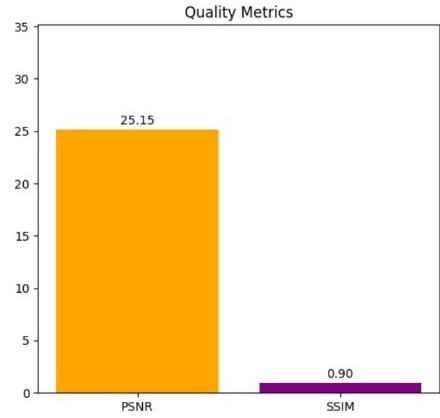
\includegraphics[width=0.6\textwidth]{image/gan.jpg} % <-- Update with your actual file path
    \caption{PSNR AND SSIM}
    \label{fig:workflow}
\end{figure}

\begin{table}[h]
\centering
\renewcommand{\arraystretch}{1.5}
\begin{tabular}{|c|c|p{8cm}|}
\hline
\textbf{PSNR (dB) Range} & \textbf{Quality} & \textbf{Description} \\
\hline
More Than 40 & Excellent & Indistinguishable from the original \\
\hline
30 -- 40 & Good & Very slight differences, barely noticeable \\
\hline
25 -- 30 & Fair / Acceptable & Noticeable noise or blur, but still usable \\
\hline
20 -- 25 & Poor & Degraded quality, visible artifacts \\
\hline
Less Than 20 & Bad & Very poor quality, heavy distortion \\
\hline
\end{tabular}
\caption{PSNR Quality Assessment range}
\end{table}

\vspace{0.5cm}
\begin{table}[h]
\centering
\renewcommand{\arraystretch}{1.5}
\begin{tabular}{|c|c|p{8cm}|}
\hline
\textbf{SSIM Value Range} & \textbf{Quality} & \textbf{Description} \\
\hline
0.95 -- 1.00 & Excellent & Structure and details very well preserved \\
\hline
0.90 -- 0.95 & Very Good & Small differences, high visual similarity \\
\hline
0.80 -- 0.90 & Good & Moderate quality, slight structural differences \\
\hline
0.60 -- 0.80 & Fair & Noticeable structural loss, acceptable in some cases \\
\hline
Less Than 0.60 & Poor & Strong structural degradation, visually different \\
\hline
\end{tabular}
\caption{SSIM Quality Assessment range}
\end{table}


% Precision, Recall, and F1 Score: For classification-based tasks such as image enhancement assessment or evaluation using a classifier.

\textbf{Image Quality Results}

From the image which compares the Original Image, the Enhanced Image, and the Quality Metrics, we extract the following:

\begin{enumerate}
    \item \textbf{PSNR: 25.15 dB}\\
    This indicates a decent level of reconstruction fidelity. Values above 25 dB are generally considered acceptable for image super-resolution, with 30+ being ideal for very high-quality reconstruction.
    
    \item \textbf{SSIM: 0.90}\\
    A high SSIM (close to 1.0) shows that the enhanced image is structurally very similar to the original HR image, indicating excellent quality preservation in terms of shapes, textures, and structural details.
\end{enumerate}

\begin{figure}[h!]
    \centering
    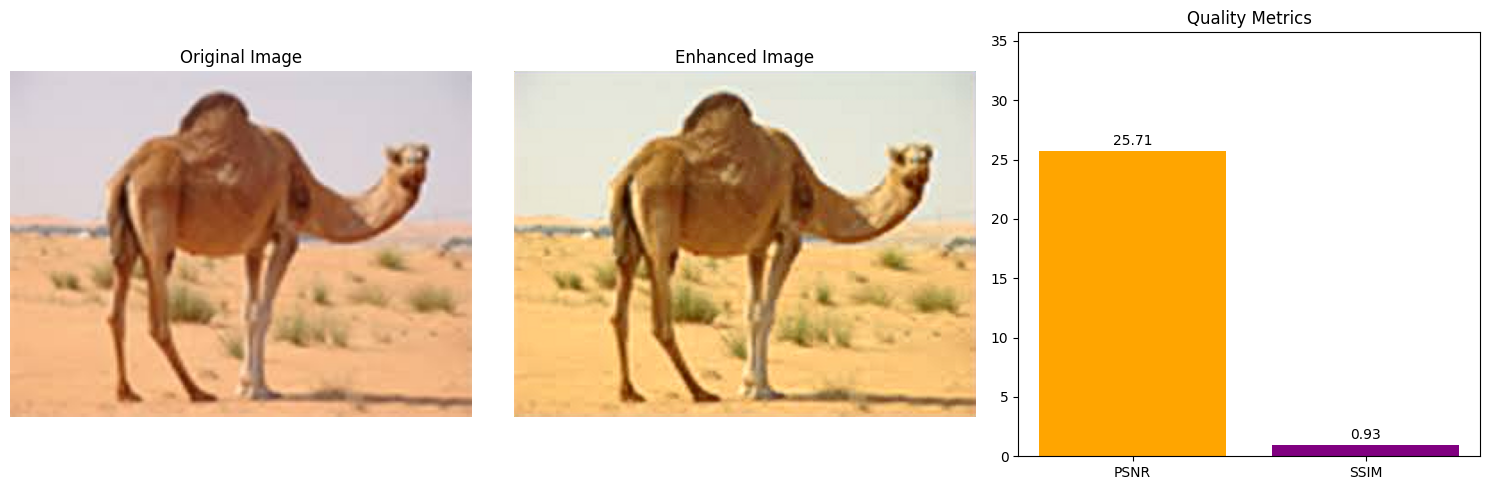
\includegraphics[width=1\textwidth]{image/ESRGAN output 4.png} % <-- Update with your actual file path
    \caption{ESRGAN Result }
    \label{fig:workflow}
\end{figure}


\notocsection{Classification-Based Evaluation}
This image provides a confusion matrix and classification metrics for some binary evaluation (likely distinguishing between high-quality vs. low-quality or real vs. generated):

\begin{table}[h]
\centering
\renewcommand{\arraystretch}{1.5}
\begin{tabularx}{0.8\textwidth} { 
  | >{\raggedright\arraybackslash}X 
  | >{\centering\arraybackslash}X 
  | >{\raggedleft\arraybackslash}X | }\hline
% \resizebox{0.9\textwidth}{!}{ % Adjust 0.9 to make it smaller or larger
\textbf{Metric} & \textbf{Value} \\
\hline
Precision & 0.8018 \vspace{0.4cm} \\
\hline

Recall    & 0.9563 \vspace{0.4cm}\\
\hline

F1 Score  & 0.8723 \vspace{0.4cm} \\
\hline
\end{tabularx}
\caption{Evaluation Metrics}
\label{tab:evaluation_metrics}
\end{table}

% \begin{figure}[h!]
%     \centering
%     
\includegraphics[width=0.93\textwidth]{image/1f1.jpg} % <-- Update with your actual file path
%     \caption{Evaluation Matrics}
%     \label{fig:workflow}
% \end{figure}
\begin{enumerate}
    \item \textbf{Precision: 0.8018}\\
    Indicates that 80.18\% of the predicted positive cases were correct.
    
    \item \textbf{Recall: 0.9563}\\
    Very high recall implies that the model was able to correctly identify most of the actual positive cases.
     
    \item \textbf{F1 Score: 0.8723}\\
    The harmonic mean of precision and recall. A high F1 score indicates a balanced and effective classification performance.
\end{enumerate}
\begin{figure}[h!]
    \centering
    \fbox{%
        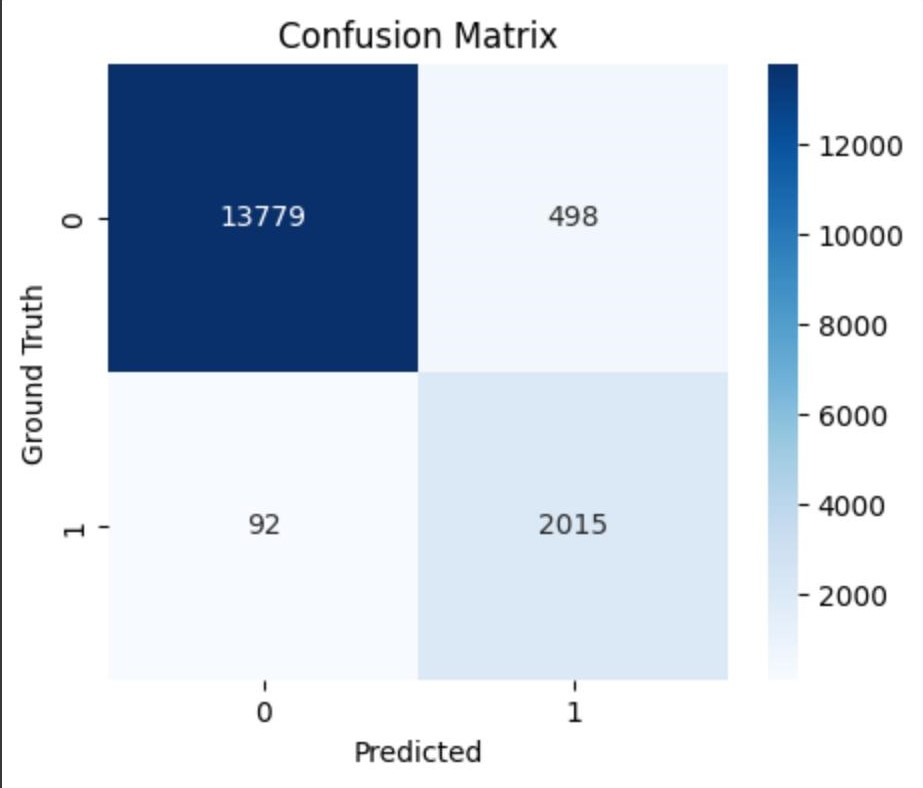
\includegraphics[width=0.6\textwidth]{image/cm.jpg} % <-- Update with your actual file path
    }
    \caption{Confusion matrix}
    \label{fig:workflow}
\end{figure}

\notocsection{Comparative Analysis: CNN vs SRGAN}
To evaluate the effectiveness of different super-resolution approaches, we compare the performance of a traditional CNN-based enhancement model and the SRGAN (Super-Resolution Generative Adversarial Network).

The comparison is based on:

\begin{itemize}
    \item Visual (Qualitative) quality
    
    \item Quantitative metrics: PSNR and SSIM
\end{itemize}

\begin{table}[h!]
    \centering
    \caption{Comparison of CNN and SRGAN Models on Image Quality Metrics}
    \resizebox{0.9\textwidth}{!}{ % Adjust 0.9 to make it smaller or larger
    \begin{tabularx}{\textwidth}{|>{\centering\arraybackslash}m{3cm}|>{\centering\arraybackslash}m{2.5cm}|>{\centering\arraybackslash}m{2.5cm}|X|}
        \hline
        \textbf{Metric} & \textbf{CNN Model} & \textbf{SRGAN Model} & \textbf{Interpretation} \\
        \hline
        PSNR (dB) & 7.09 & 25.15 & SRGAN has a significantly higher PSNR, indicating far less distortion and better image reconstruction. \\
        \hline
        SSIM & 0.18 & 0.90 & SRGAN's structural similarity to the original image is much higher, showing it retains textures and details far better. \\
        \hline
    \end{tabularx}
    }
\end{table}

% \begin{table}[h]
% \centering
% \caption{Evaluation Metrics}
%  \resizebox{0.6\textwidth}{!}{ % Adjust 0.9 to make it smaller or larger

% \begin{tabularx}{\textwidth}{|>{\centering\arraybackslash}m{3cm}|>{\centering\arraybackslash}m{2.5cm}|>{\centering\arraybackslash}m{2.5cm}|X|}\hline
% % \resizebox{0.9\textwidth}{!}{ % Adjust 0.9 to make it smaller or larger
% \textbf{Metric} & \textbf{Value} \\
% \hline
% Precision & 0.8018 \\
% Recall    & 0.9563 \\
% F1 Score  & 0.8723 \\
% \hline
% \end{tabularx}
% }
% % \label{tab:evaluation_metrics}
% \end{table}




In terms of quantitative performance, the SRGAN model significantly outperforms the CNN-based enhancement model. The Peak Signal-to-Noise Ratio (PSNR) of the CNN model is recorded at just 7.09 dB, indicating a high level of distortion in the reconstructed image. In contrast, the SRGAN model achieves a PSNR of 25.15 dB, reflecting much better reconstruction quality with reduced noise and artifacts. Similarly, the Structural Similarity Index (SSIM), which measures the perceptual similarity between the original and enhanced images, is only 0.18 for the CNN output, suggesting a poor structural match. The SRGAN output, however, attains an SSIM of 0.90, demonstrating excellent preservation of structural details and textures. 
% These metrics clearly indicate that SRGAN is more effective in producing high-quality, perceptually faithful images compared to the CNN-based approach.




\begin{figure}[h!]
    \centering
    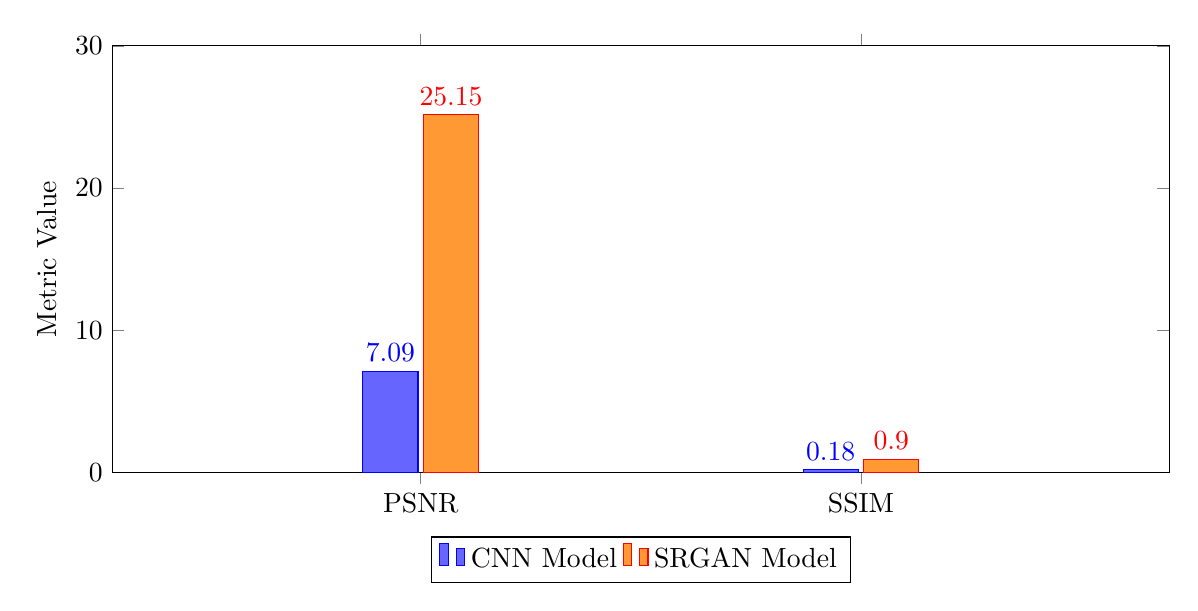
\begin{tikzpicture}
        \begin{axis}[
            ybar,
            bar width=.7cm,
            width=15cm,
            height=7cm,
            enlarge x limits=0.7,
            legend style={at={(0.5,-0.15)},
                anchor=north,legend columns=-1},
            ylabel={Metric Value},
            symbolic x coords={PSNR, SSIM},
            xtick=data,
            nodes near coords,
            nodes near coords align={vertical},
            ymin=0,
            ymax=30
        ]
        \addplot+[style={fill=blue!60}] coordinates {(PSNR,7.09) (SSIM,0.18)};
        \addplot+[style={fill=orange!80}] coordinates {(PSNR,25.15) (SSIM,0.90)};
        \legend{CNN Model, SRGAN Model}
        \end{axis}
    \end{tikzpicture}
    \caption{Comparison of CNN and SRGAN Models on PSNR and SSIM}
    \label{fig:cnn_vs_srgan_chart}
\end{figure}


\notocsection{Qualitative (Visual) Comparison}
\textbf{CNN-Enhanced Image}
\begin{itemize}
    \item Appears dark, heavily distorted, and visually degraded.
    
    \item Critical features such as facial details, hands, and food items are poorly reconstructed.
    
    \item Overall perceptual quality is very low, making the image almost unrecognizable.
\end{itemize}

\textbf{SRGAN-Enhanced Image }
\begin{itemize}
    \item Retains fine details such as facial lines, hand shape, and hair texture.
     
    \item The color distribution and contrast are more natural.
    
    \item Very close in appearance to the original image, showing excellent visual fidelity.
\end{itemize}

\vspace{0.7cm}

\begin{figure}[h]
    \centering
    
\includegraphics[width=0.3\textwidth]{image/org.jpg}
    \hfill
    
\includegraphics[width=0.3\textwidth]{image/gan1.jpg}
    \hfill
    
\includegraphics[width=0.3\textwidth]{image/cnn.jpg}
    \caption{a) Original image b) SRGAN-Enhanced Image c) CNN Enhanced Image}
    \label{fig:three_image}
\end{figure}
\begin{figure}[h!]
    \centering
    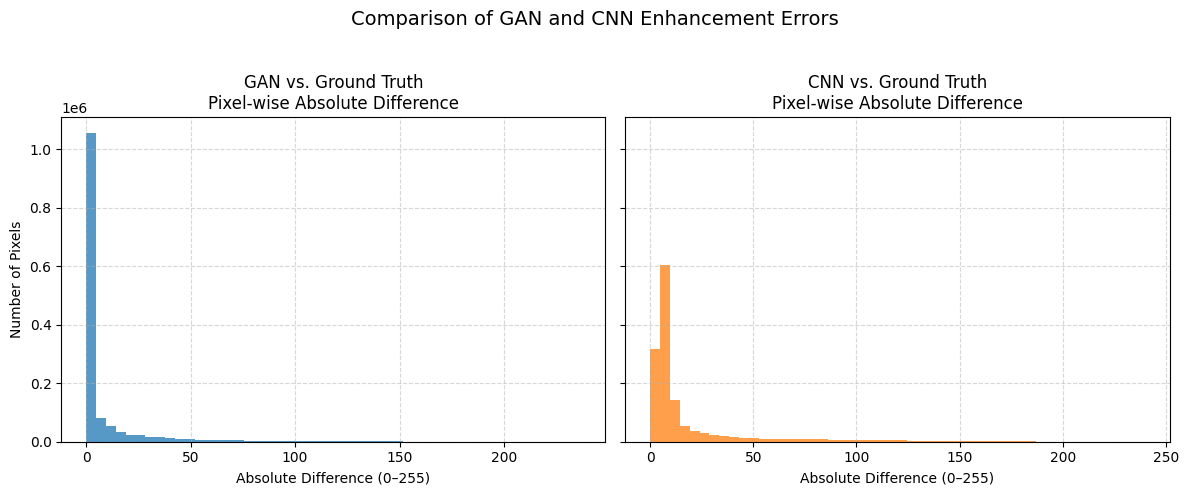
\includegraphics[width=1\textwidth]{image/download.png} % <-- Update with your actual file path
    \caption{Pixel-wise absolute difference}
    \label{fig:workflow}
\end{figure}
\textbf{Interpretation}
\begin{itemize}
    \item Histogram peak near 0 indicates many pixels match the ground truth closely.
    
    \item A narrower GAN histogram (taller near 0, shorter tails) means GAN produces fewer large errors.

    \item A wider CNN histogram (more mass at higher differences) shows CNN struggles to match fine details.
    \end{itemize}
    Visually, SRGAN produces an image nearly identical to the original, whereas the CNN model fails to reconstruct important image details.






% \begin{figure}[h!]
%     \centering
%     \begin{subfigure}[b]{0.45\textwidth}
%         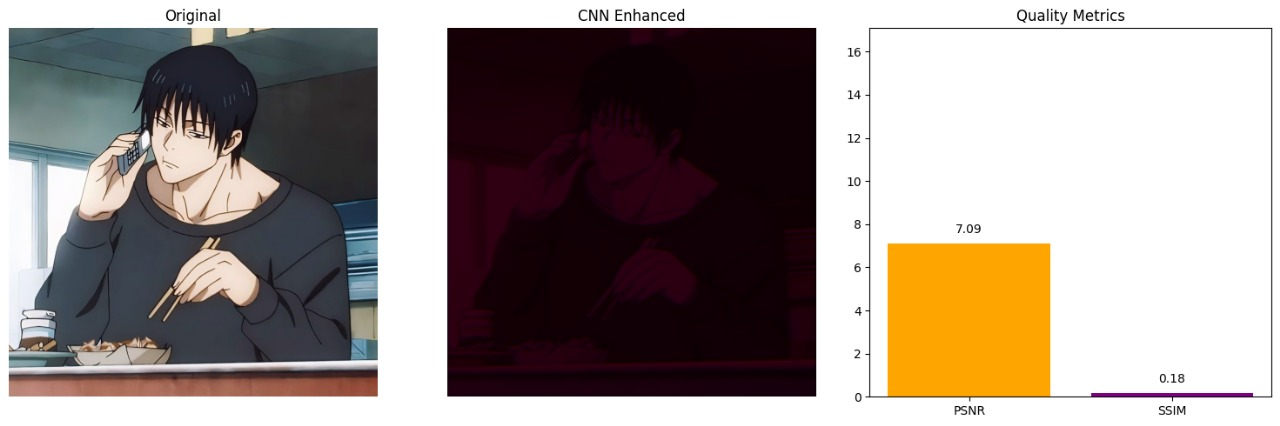
\includegraphics[width=\textwidth]{image/cnn1.jpg}
%         \caption{First Image}
%         \label{fig:image1}
%     \end{subfigure}
%     \hspace{1cm} % Adjust space between images
%     \begin{subfigure}[b]{0.45\textwidth}
%         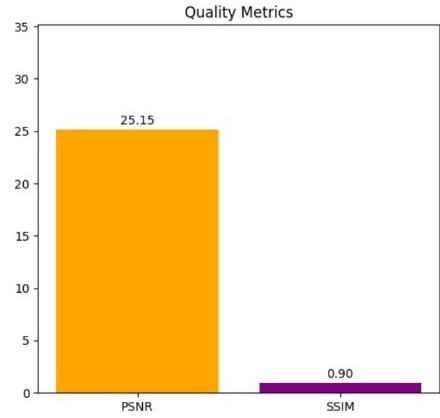
\includegraphics[width=\textwidth]{image/gan.jpg}
%         \caption{Second Image}
%         \label{fig:image2}
%     \end{subfigure}
%     \caption{Comparison of two images}
%     \label{fig:side_by_side}
% \end{figure}





















% \begin{figure}[htbp]
%     \centering
%     \begin{subfigure}[b]{0.22\textwidth}
%         \includegraphics[width=\textwidth]{r1.jpg}
%         \caption{Result 1}
%     \end{subfigure}
%     \begin{subfigure}[b]{0.22\textwidth}
%         \includegraphics[width=\textwidth]{r2.jpg}
%         \caption{Result 2}
%     \end{subfigure}
%     \begin{subfigure}[b]{0.22\textwidth}
%         \includegraphics[width=\textwidth]{r3.jpg}
%         \caption{Result 3}
%     \end{subfigure}
%     \begin{subfigure}[b]{0.22\textwidth}
%         \includegraphics[width=\textwidth]{r4.jpg}
%         \caption{Result 4}
%     \end{subfigure}
    
%     \vspace{0.5cm}
    
%     \begin{subfigure}[b]{0.22\textwidth}
%         \includegraphics[width=\textwidth]{r5.jpg}
%         \caption{Result 5}
%     \end{subfigure}
%     \begin{subfigure}[b]{0.22\textwidth}
%         \includegraphics[width=\textwidth]{r6.jpg}
%         \caption{Result 6}
%     \end{subfigure}
%     \begin{subfigure}[b]{0.22\textwidth}
%         \includegraphics[width=\textwidth]{r7.jpg}
%         \caption{Result 7}
%     \end{subfigure}
%     \begin{subfigure}[b]{0.22\textwidth}
%         \includegraphics[width=\textwidth]{r8.jpg}
%         \caption{Result 8}
%     \end{subfigure}
    
%     \caption{Super-resolution results generated by the proposed GAN model.}
%     \label{fig:results}
% \end{figure}



\chapter{Conclusion and Future Work}
In this project, we implemented and compared image super-resolution techniques using Convolutional Neural Networks (CNNs) and Generative Adversarial Networks (GANs), specifically the SRGAN architecture. Our evaluation clearly demonstrates that SRGAN significantly outperforms the CNN-based approach in terms of visual quality and quantitative performance. The SRGAN model achieved higher values of key quality metrics, including a PSNR of 25.15 dB and an SSIM of 0.90, compared to the CNN model, which yielded a PSNR of 7.09 dB and an SSIM of 0.18. This indicates that SRGAN is not only better at reducing noise and artifacts but also excels at preserving structural details and generating perceptually realistic images.

For future work, we aim to further enhance the quality of the generated images by exploring more advanced GAN architectures such as ESRGAN and Real-ESRGAN, which are known to improve fine texture recovery. Additionally, incorporating perceptual loss functions and attention mechanisms could help focus the model on more relevant features, potentially increasing PSNR and SSIM scores even further. We also plan to test our model on larger and more diverse datasets to ensure robustness and generalization. Overall, this work provides a solid foundation for high-quality image super-resolution and opens up possibilities for real-world applications such as medical imaging, satellite imagery, and video enhancement.

% ----------------- References Section -----------------
% \bibliographystyle{ieeetr}  % or try plain, unsrt, IEEEtran, etc.
\printbibliography

\end{document}
